\chapter{Introduction}

%%%%%%%%%%%%%%%%%%%%%%%%%%%%%%%%%%%%%%%%%%%%%%%%%%%%%%%%%%%%%%%%%%%%%%%%%%%%%%%%%%%%%%%%%%%%%%%%%%%%

\section{Objectives}

The primary objective of this project was to evaluate the usefulness of the Robot Operating System (ROS) \cite{ros_site} as a framework for developing complex robotic systems. Specifically, we looked to explore the variety of standard that ROS provides, in addition to the large set of community-provided packages. These packages provide a large of range of functionalities, ranging from device drivers for particular sets of sensors, to simulation suites, to full autonomous navigation suites.

As a secondary objective, we aimed to evaluate the usefulness of open-source software as a means for accelerating development of these complex systems. Additionally, by using this open-source software in the project, we set out to contribute in-kind by making any developments open-source.

%%%%%%%%%%%%%%%%%%%%%%%%%%%%%%%%%%%%%%%%%%%%%%%%%%%%%%%%%%%%%%%%%%%%%%%%%%%%%%%%%%%%%%%%%%%%%%%%%%%%

\section{Achievements}
Through the use of ROS, we will show that it was possible to implement complex behaviours such environment mapping and autonomous navigation, achieved with relative simplicity. Almost all functionality for these behaviours were is by a these standard and community-provided packages. In particular, the robot is able to walk using standard walk gaits, detect an interpret the environment around it, and navigate around that environment while avoiding any obstacles.

\begin{figure}[!h]
    \centering
    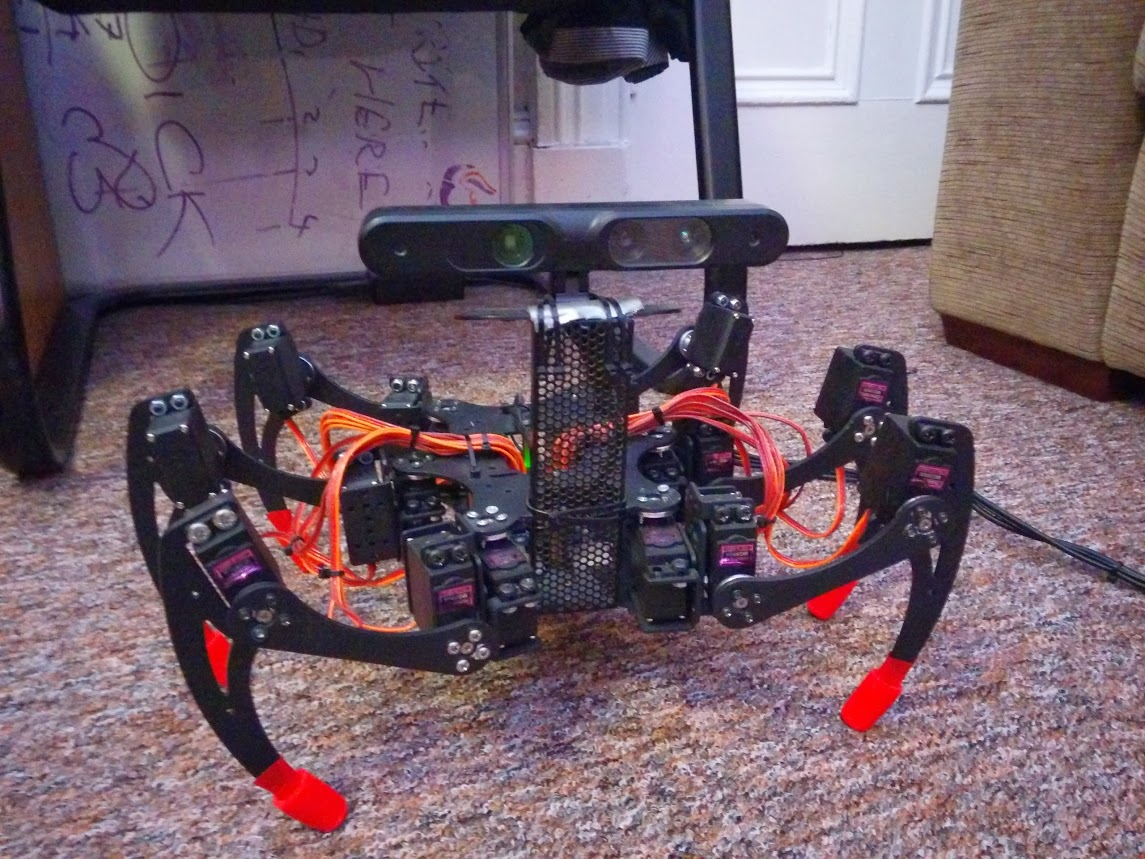
\includegraphics[width=12cm]{hexapod_body1}
    \caption{This hexapod was used as the target hardware platform for this project.}
\end{figure}

Furthermore, we show that non-standard hardware, such as the robot used throughout this project, can be integrated with ROS with relative ease. Most examples of robots running ROS tend to move themselves using either wheels or tracks, but in this case a walker-style robot is used.

%%%%%%%%%%%%%%%%%%%%%%%%%%%%%%%%%%%%%%%%%%%%%%%%%%%%%%%%%%%%%%%%%%%%%%%%%%%%%%%%%%%%%%%%%%%%%%%%%%%%

\section{Ramifications}